\documentclass[slidetop,11pt]{beamer}
\hypersetup{pdfpagemode=FullScreen}

\usepackage{polyglossia}
\setdefaultlanguage{french}

\usepackage{xunicode,xltxtra}
%\usepackage{fontspec}
%\defaultfontfeatures{Mapping=tex-text,Scale=MatchLowercase}
\setmainfont{DejaVu Sans}
%\usepackage{graphicx}
\usepackage{url,hyperref}
%\usepackage{minted}

\useinnertheme[shadow=true]{rounded}
\useoutertheme{infolines}
\usecolortheme{dolphin}
\setbeamerfont{block title}{size={}}

\title{Les processeurs}
\subtitle{des transistors par milliards}
\author{Guilhem Saurel}
\institute{ENSEEIHT}
\date{\today}
\logo{
\includegraphics[height=0.5cm]{images/inp-enseeiht}}

\begin{document}

\frame{\titlepage}

\begin{frame}{Sommaire}
    \small \tableofcontents
\end{frame} 

\section[L'ordinateur]{De l'architecture générale au processeur}
    \subsection[UC]{L'unité centrale}
        \begin{frame}
            \frametitle{L'unité centrale}
            \begin{itemize}
                \item L'alimentation
                \item Les lecteurs de disques
                \item La carte mère
                \item Les cartes filles
            \end{itemize}
        \end{frame}
 
    \subsection[MoBo]{La carte mère}
        \begin{frame}
            \frametitle{Photo}
            \begin{center}
                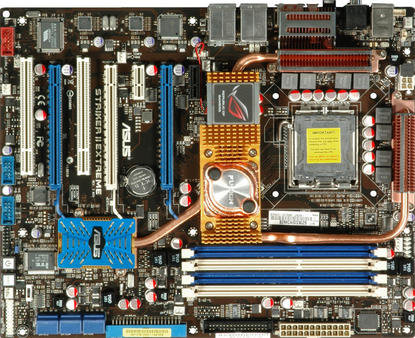
\includegraphics[height=6.5cm]{images/mobo}
            \end{center}
        \end{frame}
 
        \begin{frame}
            \frametitle{Architecture}
            \begin{center}
                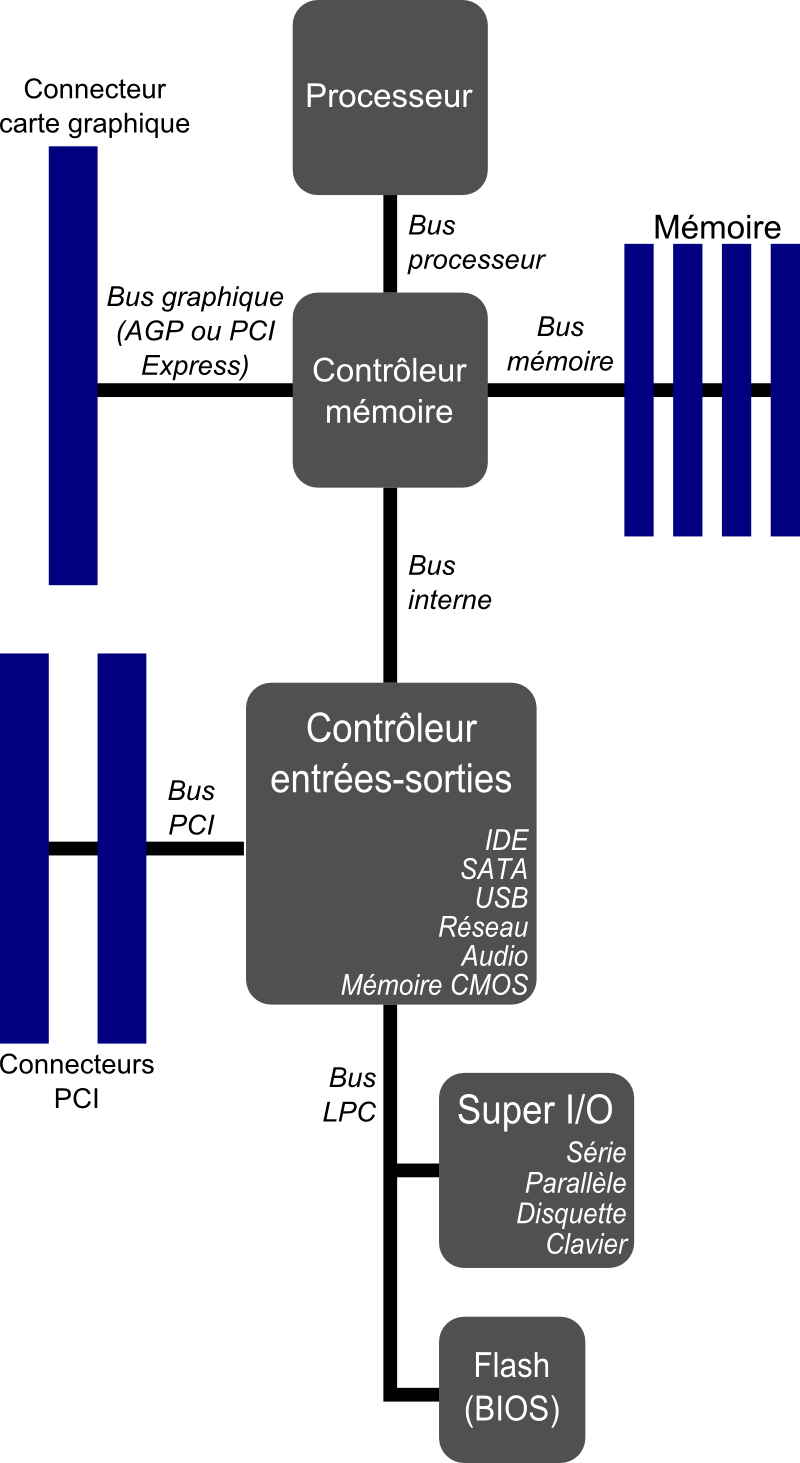
\includegraphics[height=6.5cm]{images/mobo_arch}
            \end{center}
        \end{frame}
 
%TODO transition
 
\section[Arch]{L'architecture}
    \subsection[ASM]{L'assembleur}
        \begin{frame}
            \frametitle{Le jeu d'instructions d'un PIC®}
            \begin{center}
                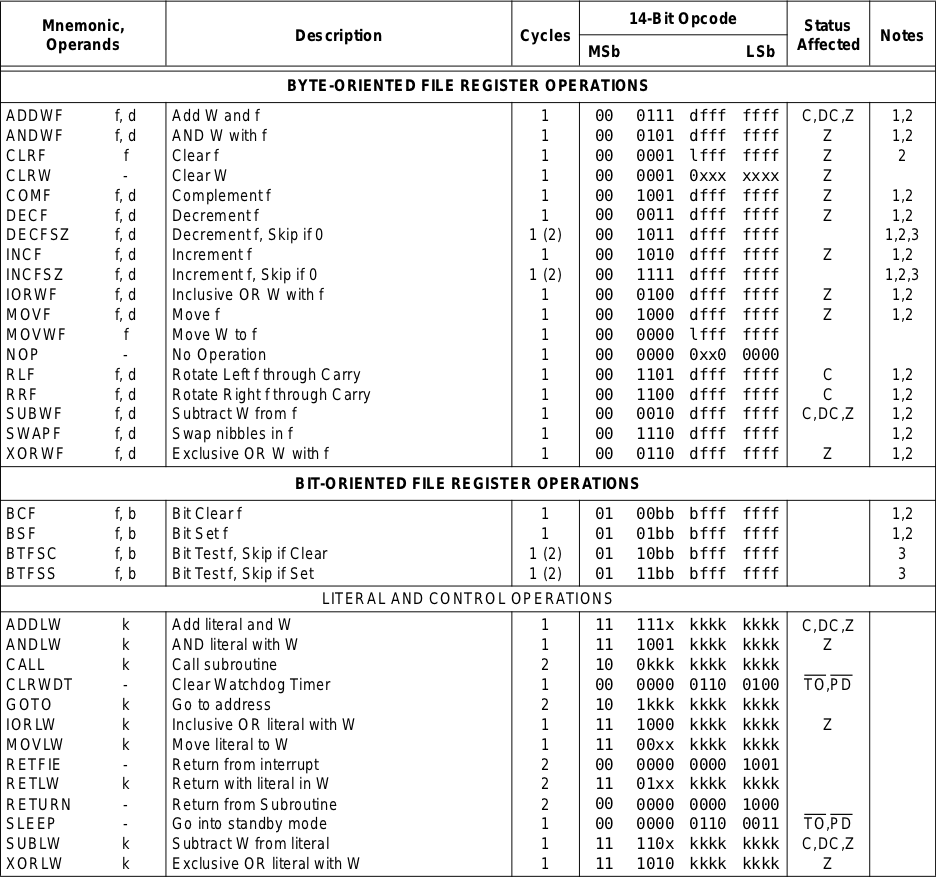
\includegraphics[height=6.5cm]{images/16f84a}
            \end{center}
        \end{frame}
  
    \subsection[ISA]{Les jeux d'instructions}
        \begin{frame}
            \frametitle{RISC vs CISC}
            \begin{block}{RISC}
                \begin{itemize}
                    \item Peu d'instructions à connaitre
                    \item Code peu lisible
                \end{itemize}
            \end{block}
            \begin{block}{CISC}
                \begin{itemize}
                    \item Instructions très complexes => très puissantes
                    \item Complexité de conception du processeur et des compilateurs
                \end{itemize}
            \end{block}
        \end{frame}
  
        \begin{frame}
            \frametitle{Exemples}
            \begin{itemize}
                \item ARM
                \item PowerPC
                \item x86
                \item Sparc
            \end{itemize}
        \end{frame}
  
    \subsection[Fonctionnement]{Fonctionnement}
        \begin{frame}
            \frametitle{Le schéma de fonctionnement d'un PIC®}
            \begin{center}
                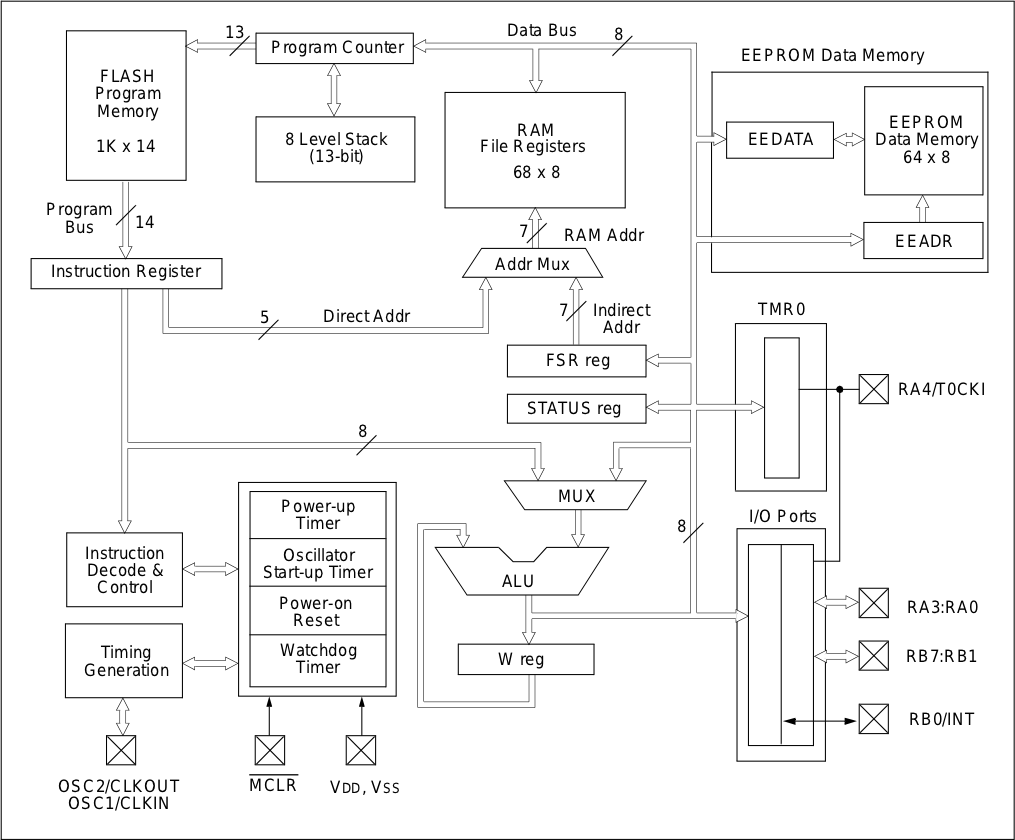
\includegraphics[height=6.5cm]{images/arch.png}
            \end{center}
        \end{frame}
 
        \begin{frame}
            \frametitle{Les composants}
            \begin{itemize}
                \item L'horloge
                \item L'unité arithmétique et logique
                \item L'unité d'entrées-sorties
                \item Le séquenceur
                \item Les registres
            \end{itemize}
        \end{frame}
 
    \subsection[Pipeline]{Le Pipeline}
        \begin{frame}
            \frametitle{Cas d'un CISC qui a besoin de 5 cycles pour 1 instruction}
            \begin{center}
                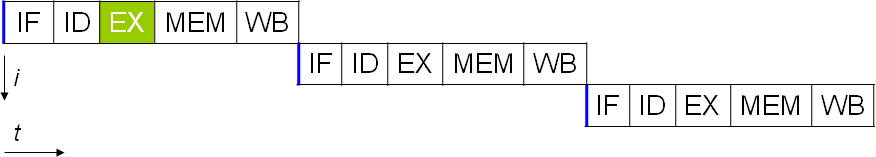
\includegraphics[width=\linewidth]{images/Nopipeline}
            \end{center}
        \end{frame}

        \begin{frame}
            \frametitle{Pipeline à 5 étages}
            \begin{center}
                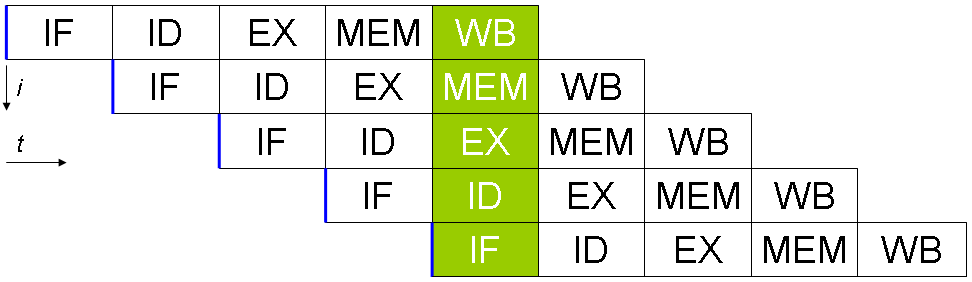
\includegraphics[width=\linewidth]{images/Fivestagespipeline}
            \end{center}
        \end{frame}

        \begin{frame}
            \frametitle{Pipeline à 5 étages superscalaire}
            \begin{center}
                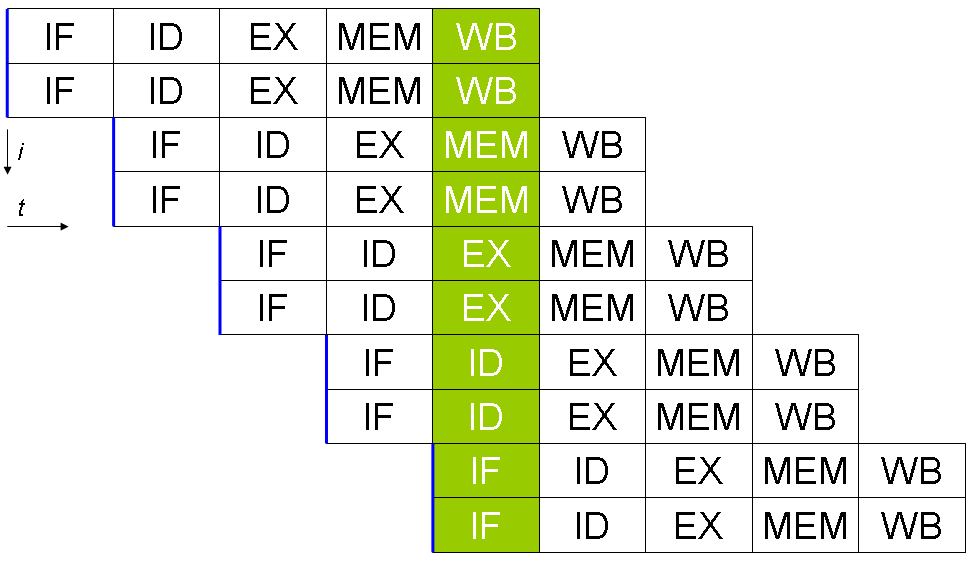
\includegraphics[height=6.5cm]{images/Superscalarpipeline}
            \end{center}
        \end{frame}

%TODO transition

\section[Hardware]{Un exemple d'implémentation matérielle}
    \begin{frame}
        \frametitle{NVIDIA Tegra 2}
        \begin{center}
            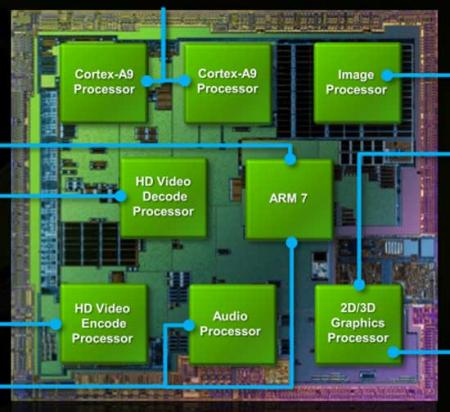
\includegraphics[height=6.5cm]{images/tegra}
        \end{center}
    \end{frame}

\section[CPU]{Un exemple de processeur complet}
    \begin{frame}
        \frametitle{Un CPU open source : l'UltraSPARC T2}
        \begin{center}
            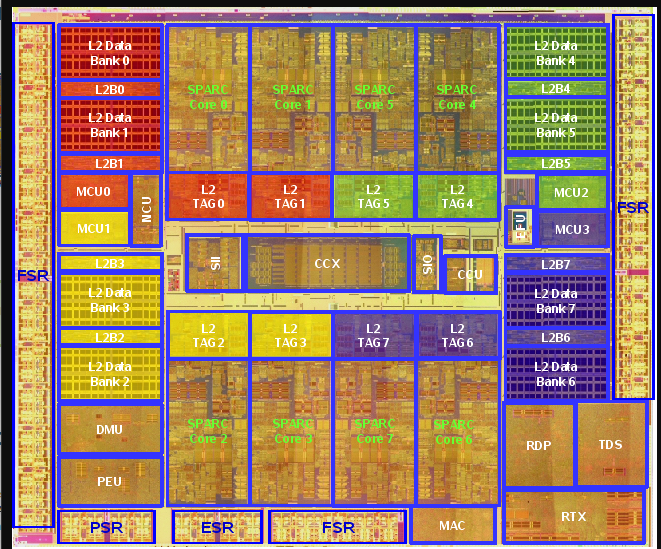
\includegraphics[height=6.5cm]{images/T2}
        \end{center}
    \end{frame}

\end{document}
